% ============================================================================================
% This is a LaTeX template used for the course
%
%  I M A G E   B A S E D   B I O M E T R I C S
%
% Faculty of Computer and Information Science
% University of Ljubljana
% Slovenia, EU
%
% You can use this template for whatever reason you like.
% If you have any questions feel free to contact
% ziga.emersic@fri.uni-lj.si
% ============================================================================================

\documentclass[9pt]{IEEEtran}

% basic
\usepackage[english]{babel}
\usepackage{graphicx,epstopdf,fancyhdr,amsmath,amsthm,amssymb,url,array,textcomp,svg,listings,hyperref,xcolor,colortbl,float,gensymb,longtable,supertabular,multicol,placeins}

 % `sumniki' in names
\usepackage[utf8x]{inputenc}

 % search and copy for `sumniki'
\usepackage[T1]{fontenc}
\usepackage{lmodern}
\input{glyphtounicode}
\pdfgentounicode=1

% tidy figures
\graphicspath{{./figures/}}
\DeclareGraphicsExtensions{.pdf,.png,.jpg,.eps}

% correct bad hyphenation here
\hyphenation{op-tical net-works semi-conduc-tor trig-gs}

% ============================================================================================

\title{\vspace{0ex} %
% TITLE IN HERE:
Iris Feature Extraction Using Convolutional Neural Networks
\\ \large{Research seminar}\\ \normalsize{Image Based Biometry 2020/21, Faculty of Computer and Information Science, University of Ljubljana}}
\author{ %
% AUTHOR IN HERE:
Andrej~Hafner
\vspace{-4.0ex}
}

% ============================================================================================

\begin{document}

\maketitle

\begin{abstract}
Iris recognition refers to the automated process of individual recognition based on the patterns in their irises. Due to its uniqueness it's a common modality used in biometric recognition. With a technique pioneered by Daugman, it was shown that it enables recognition with very low false match rates. We adapt the pipeline defined by Daugman and introduce convolutional neural networks (CNN) to function as feature extractors. We train the CNNs on a part of CASIA-Iris-Thousand dataset for closed set prediction. Trained models are then used as feature extractor, which are used in recognition. With DenseNet-201 we achieve $97.3\%$ recognition accuracy in closed set recognition and $98.5\%$ recognition accuracy in open set recognition.
\end{abstract}

\section{Introduction}
Iris recognition is a process, in which an individual is identified with the use of patterns in their irises. Uniqueness of the iris is crucial, since this enables us to uniquely identify an individual. In this work we adapt the traditional pipeline invented by Daugman \cite{daugman2009iris}. We use convolutional neural network (CNN) for closed and open set iris recognition. In closed set recognition CNN are trained and then used to predict the identity of the user. Since this approach is impractical in real life system, we focus on open set recognition, where templates are easily added to the database, without the need for model retraining. In open set recognition we use CNNs, trained on closed set, as feature extractors. We recognize subjects by calculating cosine similarity between the feature vectors. Models are trained and evaluated on the CASIA-Iris-Thousand database. We start by an overview of related works and then continue to the methodology, where we describe the dataset, define the recognition pipeline and set up the experimental protocol. In results we first describe the metrics used for evaluation and then discuss the results of closed and open set recognition.

\section{Related works}
We can attribute the success of iris recognition to the development of efficient feature descriptors. The first descriptors, developed by Daugman \cite{daugman2009iris}, achieved  really good results and are still in use today in many systems worldwide. He used Gabor phase-quadrant feature descriptor on a segmented and normalized image of the iris. He matched the descriptors using Hamming distance.

Other handcrafted feature descriptors were also used, such as Discrete Fourier transforms (DFT) \cite{miyazawa2008effective} and class-specific weight maps, learned from the images of the same class \cite{dong2010iris}. Authors of \cite{nguyen2017iris} used off-the-shelf CNNs to extract feature vectors, which were then used to train support vector machine (SVM). They extracted features from different layers throughout the neural network and achieved best performance using outputs from the layers in the middle. In \cite{boyd2020deep} authors compare the approaches of feature extraction using CNNs for iris recognition. They compared the performance of using existing models, training them from scratch or finetuning. Feature dimensionality was reduced using principal component analysis (PCA) and the outputs were fed to a one-versus-rest SVM for classification. They achieved best results using finetuned models, the approach we also use in this research.


\section{Methodology}
In this chapter we first describe the iris dataset used. We continue with the description of CNNs used and their function as feature extractors. Next, we define the recognition pipeline and explain the difference between open and closed set recognition. We finish the chapter with the definition of the experimental protocol applied.

\subsection{Dataset}
CASIA-Iris-Thousand is an iris dataset collected by the Chinese Academy of Sciences Institute of Automation (CASIA) \cite{casia-iris-thousand}. It contains 20000 iris images from 1000 subjects, collected by an IKEMB-100 camera in near-infrared spectrum (NIR). There are 10 left and 10 right eye images for each subject, some containing eyeglasses and specular reflections, which increases the intra-class variation. Since each iris is considered to be unique (of the same person), we define the image of a specific eye as it's own class, thus acquiring 2000 classes from the dataset. Size of the images is $640\times480$. We can see two examples from the dataset in figure (\ref{fig:casia-example}).
\begin{figure}[h]
    \centering
    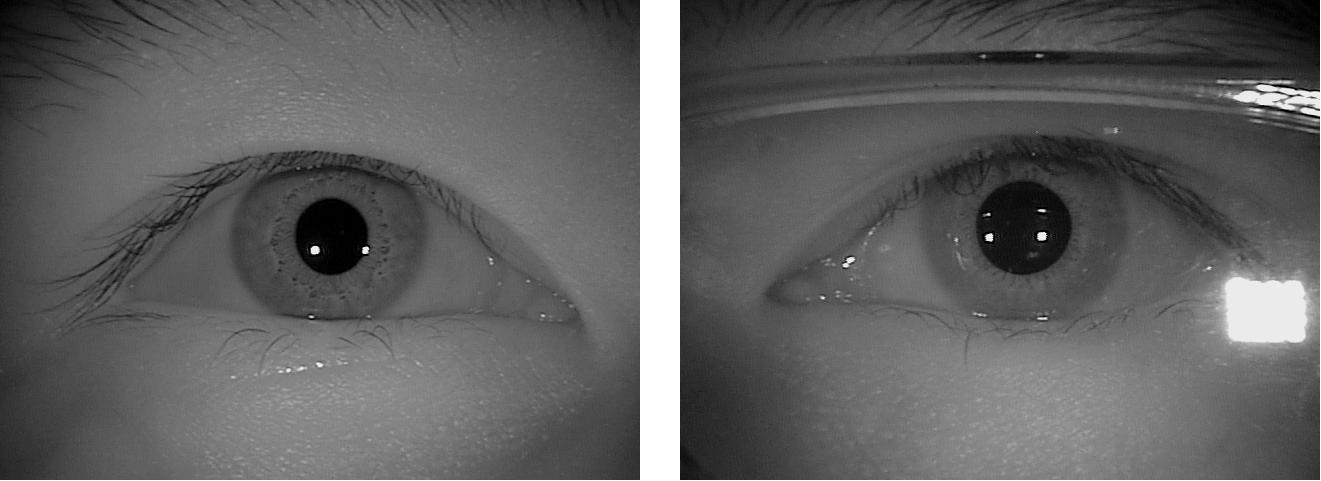
\includegraphics[width=1\columnwidth]{figures/casia-iris-thousand-example.png}
    \caption{Example images from the CASIA-Iris-Thousand dataset. Images are from left and right eye of two different subjects. The subject on the right is wearing glasses.}
    \label{fig:casia-example}
\end{figure}

\subsection{CNNs and feature extraction}
CNNs have been dominating the field of computer vision. In this research we use ResNet-101 \cite{resnet} and DenseNet-201 \cite{densenet} architectures, both intended for image classification tasks. ResNet introduces the concept of skip or residual connections, where the outputs skip a layer and are feed into the next layer. This helps solve the problem of vanishing gradients. DenseNet utilizes the concept of densely connected layers. Each layer obtains additional inputs from all the preceding layers and each layer also passes it's own feature maps to subsequent layers. The inputs to the layers are concatenated with the passed feature maps. This enables the network to be more compact, increasing the computational and memory efficiency.

We use finetuning to train our models. In finetuning, we initialize our models with pretrained weights, trained on a different dataset. This helps the models to learn faster and achieve better accuracy, since the earlier layers already contain filters, trained to detect edges and color blobs, which are present in most of the images. It is also a better approach, when we don't have a sufficient amount of data, which is true in our case (10 images per class) \cite{cadene2016master}. Both of our architectures were pretrained on ImageNet dataset \cite{imagenet_cvpr09}. Because of this, their final layers contain 1000 outputs, since the ImageNet dataset contains 1000 classes. We reshaped the final layers of both networks to match the number of classes in our closed dataset, which we describe in chapter (\ref{exp_prot}).

Once trained on a closed set, CNNs can function as feature extractors. The output of each layer is a descriptor of the input to the network. The earlier layers retain coarser information and the later layers finer and more abstract information. In both architectures we flatten the output of the last average pooling layer, receiving a 2048-dimensional feature vector. 

\subsection{Recognition pipeline}
We define two recognition pipelines, first one for closed set recognition and second one for open set recognition. Closed set recognition is when we recognize only the identities which were used in training for our models. Recognition is done by inputting the preprocessed iris image to the model, then the identity is found by finding the maximum output on the final layer. This creates a problem, since adding a new identity would require reshaping the final layer and retraining the network. This wouldn't be practical in a real life system, where many identities could be enrolled on a daily basis. To solve this problem, we use our trained models as feature extractors, which enables us to do open set recognition. We extract a feature vector from the input of the image, which is used as an identifier for the class and enrolled to a database. When doing recognition, we again pass the iris image to the model and extract the feature vector. We compute the similarity between this vector and all the vectors enrolled in our database. Recognition is done by finding the subject, which has the corresponding vector with the highest similarity to the vector we retrieved from the model. This enables us to easily enroll new identities to our database, without retraining the models.

First stage of recognition is shared by both pipelines, which we can see in the figure (\ref{fig:iris-pipeline}). We use a similar approach to traditional iris recognition, first defined by Daugman \cite{daugman2009iris}. Modified method was defined by the authors of \cite{USIT2} and the code was taken from their GitHub repository. Iris is first segmented from the image using weighted adaptive Hough transform and ellipsopolar transform (\textit{wahet}). We normalize the segmented iris to size $256\times64$. Next, we enhance the normalized image by increasing the contrast between the lighter and darker areas. This accentuates the features of the iris that make it unique. We then stack copies of the enhanced image on top of each other four times, getting an image of size $256\times256$. This enables us to get a square image, which is required by the model. Finally we resize the image to the input size of $224\times224$.

\begin{figure}[h]
    \centering
    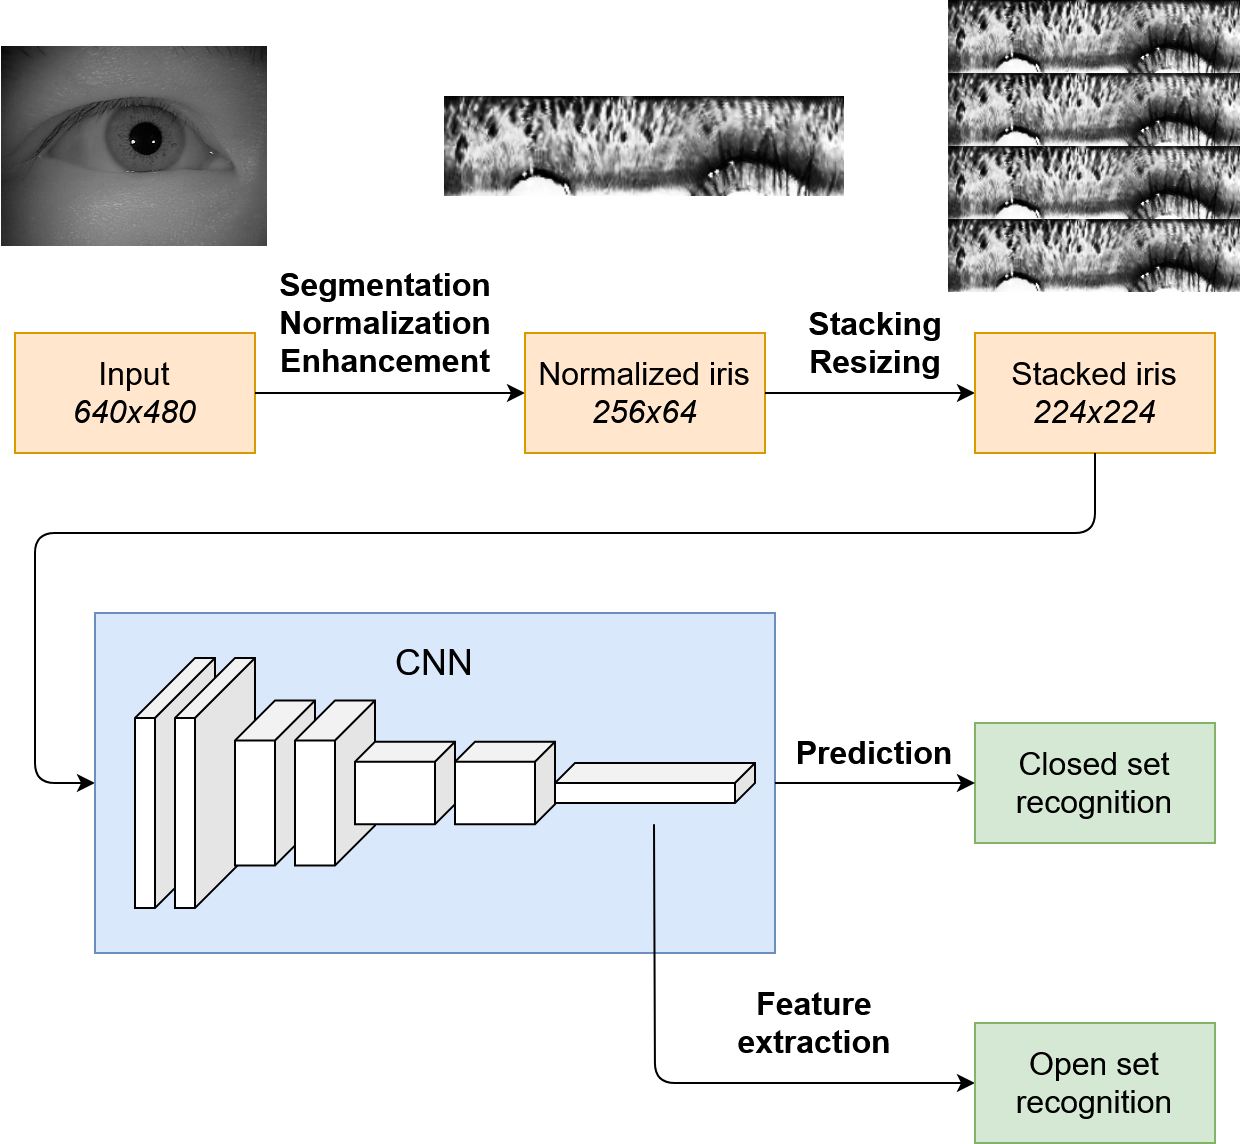
\includegraphics[width=1\columnwidth]{figures/iris-cnn-pipeline-compact.png}
    \caption{Iris recognition pipeline for open and closed sets. Iris is segmented from the image using weighted adaptive Hough transform and ellipsopolar transform, then normalized to a size of $256\times64$. We then increase the contrast in the image to accentuate the features of the iris. Output is then stacked on top of each other four times in order to get a square image, then resized to $224\times224$, which is the size required by the CNN. CNN is then used for prediction in closed set recognition and as a feature extractor for open set recognition.}
    \label{fig:iris-pipeline}
\end{figure}

In the second stage of the pipeline we use the CNN for closed set recognition. Irises we want to identify are input to the CNN and the subject is recognized by looking for the maximum output on the final layer. For open set recognition we input the iris to the network and then take the flattened output of the last average pooling layer in both architectures as a 2048-dimensional feature vector. At enrollment phase images feature vectors are saved to a database. When trying to recognize an iris, we again feed it to the CNN and extract a feature vector. We then compute the cosine similarity (\ref{eq:cosine}) between the the latter feature vector and all of the feature vectors in the database.
\begin{equation}
\label{eq:cosine}
    cos(x, y) = \frac { x \cdot y}{||x|| \cdot ||y||}
\end{equation}
Subject that has a corresponding feature vector with the highest similarity is matched.

\subsection{Experimental protocol}
\label{exp_prot}
For our experiments we split the dataset into two parts. The first part is used for closed set recognition and to train CNNs for feature extraction. It contains 1500 classes. For each class we choose 7 images for training, 2 for validation and 1 for testing. The second part consists of 500 classes and is used for open set recognition. We use 7 images per class for enrollment into the database and 3 images per class for testing.

We trained both ResNet-101 and DenseNet-201 using Adam optimizer and categorical cross-entropy loss function. ResNet-101 was trained with learning rate $2\cdot10^{-5}$ for $80$ epochs and DenseNet-201 with learning rate $10^{-4}$ for $80$ epochs. Both models were trained on Nvidia GTX 980 Ti GPU with 8GB VRAM. Both models and their weights were taken from the Pytorch library \cite{NEURIPS2019_9015}.

For open set evaluation we used both of the models trained for closed set recognition. For each class we enroll 7 images and test the performance using 3 images. We also evaluate open set recognition using 5-fold cross validation. In each fold we enroll 8 images and use 2 for testing.

\section{Results}
In this chapter we first define the metrics used for recognition evaluation. We then present the results of the closed and open set recognition, followed by the discussion.

\subsection{Metrics}
We evaluate the performance of closed and open set recognition with rank-1 accuracy, rank-5 accuracy and with cumulative match-score curve (CMC). In closed set recognition we can apply softmax function to the outputs of the final linear layer. This gives a probability estimation for each of the classes, as the sum of the output equals 1. In open set recognition we receive cosine similarities between all the pairs and we select the highest similarity in each class (one out of seven). This way we get a similarity between the feature vector being evaluated and each of the classes. The value of cosine similarity is between 0 (vectors are orthogonal) and 1 (vectors are parallel), when vectors are normalized. Next, we order the probabilities in closed set recognition and similarities in open set recognition in descending order. Rank-1 accuracy is then defined by the number of the ground truth labels that are equal to the corresponding label of class with the highest probability or similarity, divided by the number of all test cases. We can define rang-\textit{n} accuracy in the same way, but in this case we check for equality of labels in the first \textit{n} highest probability or similarity predicted labels, again divided by the number of all test cases. This means that rank-\textit{k} accuracy, where \textit{k} is equal to the number of classes, is always equal to 100\%. We plot a CMC curve by evaluating rank-\textit{n} accuracy for ranks from 1 to number of all classes. Y axis is then the rank-\textit{n} accuracy and X axis is the rank. A CMC curve tells us how the recognition accuracy is changing with increasing ranks.

\subsection{Closed set evaluation}
Results of closed set evaluation are presented in table (\ref{tab:results-closed}).

\begin{table}[h]
    \centering
    \caption{Closed set recognition evaluation results}
    \def\arraystretch{1.3}
    \begin{tabular}{ l | c | c} 
        Model & Rank-1 accuracy & Rank-5 accuracy \\
        \hline
        DenseNet-201 & $\textbf{97.3\%}$ & $\textbf{99.3\%}$ \\
        \hline
        ResNet-101 & $96.2\%$ & $98.7\%$ \\
    \end{tabular}
    \label{tab:results-closed}
\end{table}

We can see that DenseNet-201 outperformed ResNet-101 in both rank-1 and rank-5 accuracy. Both of the models performed very well, reaching higher than $96\%$ rank-1 accuracy. In figure (\ref{fig:closed-set-cmc}) we can see, that rank-\textit{n} accuracy is increasing fast up to $\textit{n} = 6$, then it slows down. This means that most of the correct recognition's are in the first 6 highest probability predictions. At around rank-50 recognition accuracy comes really close to $100\%$. Incorrectly recognized test cases can be attributed to noisy data, which leads to mistakes in iris segmentation, as seen in figure (\ref{fig:iris-poor-images-example}).

\begin{figure}[h]
    \centering
    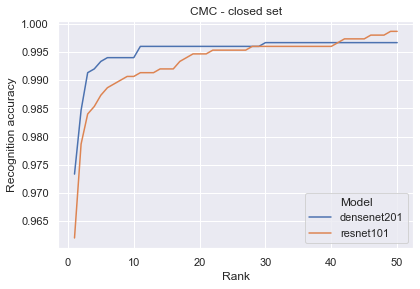
\includegraphics[width=1\columnwidth]{figures/closed_set_cmc.png}
    \caption{CMC curves from close set recognition evaluation. In the legend we can see which CMC curve belongs to the evaluation of which model. We plot CMC curves to rank 50, since the accuracy stops increasing until rank is equal to the number of all classes. It also makes the graph more readable.}
    \label{fig:closed-set-cmc}
\end{figure}

\subsection{Open set evaluation}

In open set recognition evaluation DenseNet-201 again outperforms ResNet-101 in feature extraction function of CNN (table (\ref{tab:results-open})). 

\begin{table}[h]
    \centering
    \caption{Open set recognition evaluation results}
    \def\arraystretch{1.3}
    \begin{tabular}{ l | c | c} 
        
        Model & Rank-1 accuracy & Rank-5 accuracy \\
        \hline
        DenseNet-201 & $\textbf{98.7\%}$ & $\textbf{99.6\%}$\\
        ResNet-101 & $98.4\%$ & $99.2\%$\\
        \hline
        DenseNet-201 CV & $\textbf{98.5\%}$ $(\pm0.2\%)$ & $\textbf{99.2\%}$ $(\pm0.1\%)$\\
        ResNet-101 CV & $97.7\%$ $(\pm0.3\%)$ & $98.9\%$ $(\pm0.2\%)$ \\
        
    \end{tabular}
    \label{tab:results-open}
\end{table}

In order to ensure that the test cases were not selected in such a way, that would increase the accuracy, we also cross validated both of our models (results are denoted with CV next to the model name). DenseNet-201 comes on top again, achieving almost the same accuracy as in normal testing. Standard deviation across the folds is below $0.3\%$ for both of the models, meaning that no part of the images of a certain class stands out in better or poorer performance. Same holds true across different rank-\textit{n} accuracies, as seen in CMC curves in figure (\ref{fig:open-set-cv-cmc}), where the coloured area around the curves represents the standard deviation. The authors of \cite{nguyen2017iris} used Daugman's implementation as a baseline on the CASIA-Iris-Thousand database and achieved $90.7\%$ recognition accuracy. We can compare our results to their baseline estimation, although we need to consider that they tested it on the whole database.

\begin{figure}[h]
    \centering
    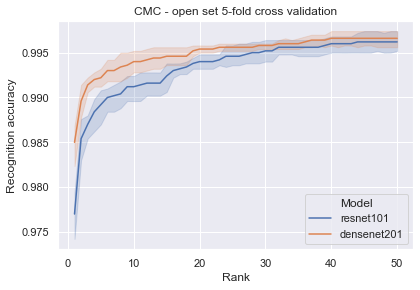
\includegraphics[width=1\columnwidth]{figures/cv_cmc.png}
    \caption{CMC curves from open set recognition cross validation. Curves belong to the models as described in the legend. Coloured area around the curve defines the standard deviation calculated between all the folds in cross validation. Values for specific rank-\textit{n} accuracies are averaged over all the folds. We plot CMC curves to rank 50, since the accuracy stops increasing until rank is equal to the number of all classes. It also makes the graph more readable.}
    \label{fig:open-set-cv-cmc}
\end{figure}

In figure (\ref{fig:open-set-cv-cmc}) we can see that even at rank $50$ we don't reach $100\%$ recognition accuracy. The reason for this are probably the glasses, that the subjects are wearing in images. In figure (\ref{fig:iris-poor-images-example}), we can see that glasses create a reflection, which intersects with the iris. This prevents the \textit{wahet} algorithm from good segmentation and normalization of the iris. In turn this leads to the CNNs extracting feature vectors from the stacked image, which are not good descriptors of the iris. We could solve this problem by increasing the robustness of the first stage in our recognition pipeline. In real life systems we could also rate the quality of segmented iris. If the quality would be too low, we would reject the recognition and ask the subject to try again.

\begin{figure}[h]
    \centering
    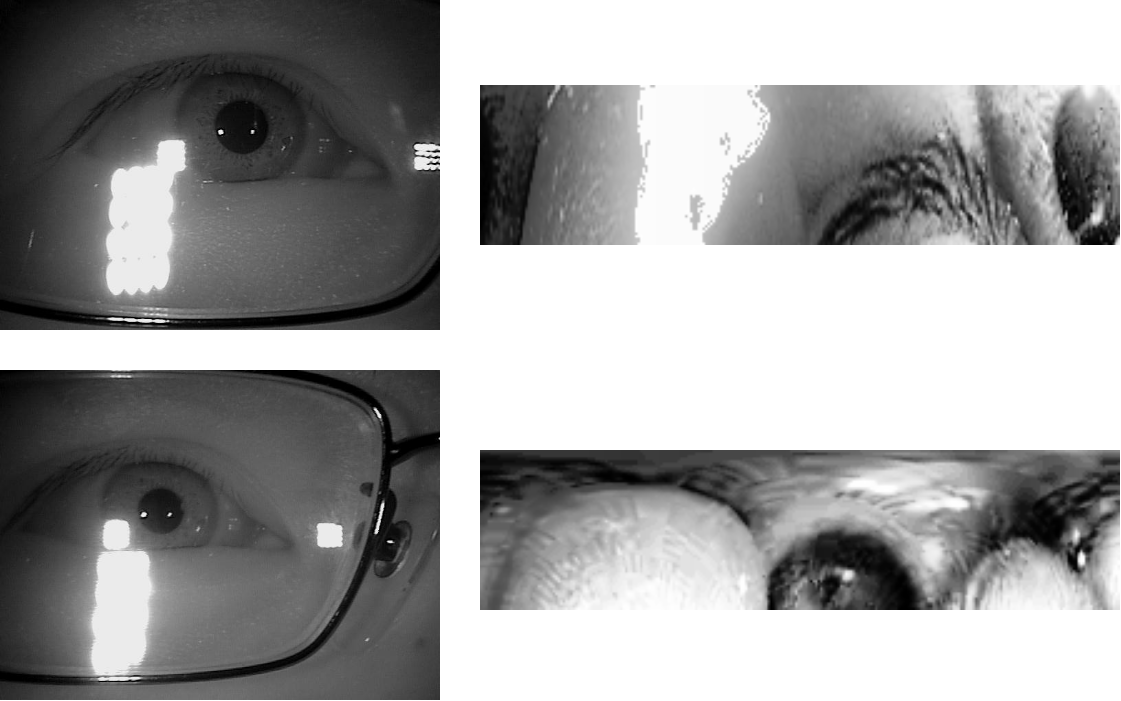
\includegraphics[width=1\columnwidth]{figures/iris-cnn-bad-segmentation.png}
    \caption{Examples of false matches in the open set recognition evaluation. Subjects in these two images are wearing glasses, which create a reflection over the iris. On the right we can see the result of segmentation, normalization and enhancement. There is almost no sign of iris structure, which makes each iris unique (we can see a good example in figure (\ref{fig:iris-pipeline})). The lack of structure prevents the CNN to extract discriminative features, thus a false match is made.}
    \label{fig:iris-poor-images-example}
\end{figure}
 

\section{Conclusion}
In this research we approach the task of iris recognition with CNNs. Irises are segmented and normalized from the images using the \textit{wahet} algorithm. We finetune DenseNet-201 and ResNet-101 on a subset of the CASIA-Iris-Thousand dataset for closed set recognition. Models are then reused as feature extractors for open set recognition. We show that finetuned CNNs can produce discriminative features, with which we can achieve very high recognition accuracy. We also show that initializing CNNs with weights pretrained on other datasest can lead to a speedup in training. It also helps if the amount of data per class is small.

We make the implementation and the models publicly available on our GitHub page \cite{andrej-github}.

\bibliographystyle{IEEEtran}
\bibliography{bibliography}

\end{document}